% todo CM in extra figures
\part{The final model}
\label{part:final_model}

%------------------------------------

\section{About this part}
\label{section:opt_about_part}

Whilst a great insight on the working of different models and a typical AI pipeline has been achieved with the experiments discussed so far, many things were left unexplored.
This is mostly due to limited computational power and time available.
A final attempt is made to make a better performing model using the further insight received from experiments up until now.
Things that were not tried but which are \textit{assumed} to increase performance are also listed here.
This part will only briefly discuss all steps to avoid repetition and an even longer document. 
The Notebooks corresponding with this part are \texttt{final\_model\_exploration.ipynb}, \texttt{final\_model.ipynb}, \texttt{svc\_large.ipynb},  \texttt{clustering.ipynb} and \texttt{more\_helpers.py}.
The Notebooks provide inline comments on the found results.

%------------------------------------

\section{Making a better individual model}
\label{section:opt_better_model}

Firstly, some of the made decisions early on, such as the used descriptor and cluster amount, are reconsidered.
The following things were tried to make a better performing LBM and SVC model: 
\begin{itemize}
    \item Different scalers and transformers were tried as preprocessing (after clustering). The SVC model did not benefit from this but applying the polynomial features transformer on the LBM model significantly increased the performance by 0.1 on the test set and Kaggle (now 1.57203)!
    \item The train set was balanced and overfitted, neither of which increased global or individual performance. The balanced train set does give a more representative MCLL score and thus will be used to determine the weighted probabilities for the final model.
    \item Neither \texttt{AdaBoostClassifier} or the \texttt{BaggingClassifier} to make an ensemble of the LBM and SCV models performed well. This can be expected since such ensembles work well when combining \textit{weak models}, which SVC and the LBM are not.
    \item The SIFT descriptor with 100 clusters was used as the default for this report, this is now reconsidered by testing SVC with more clusters. It was found that giving SVC more clusters drastically improved its performance without seeming to lose generality based on the confusion matrix. 1250 clusters seemed optimal.
    \item The \texttt{createCodebook} helper function uses \texttt{MiniBatchKMeans} for a given cluster amount, according to \citet{kmeansvsmini}, using this faster variant over regular K-Means results in worse performance. This was explored and it was found opting for regular K-Means does indeed increase model performance, all be it with the cost of a tremendous slower clustering. Some different clustering algorithms, such as \texttt{GaussianMixture} were also tried, but this didn't yield an increase in performance.
    \item Preprocessing after and before clustering was also considered. One of which is using \textit{RootSIFT} as proposed by \citet{rootsift}. Opting to use root-sift combined with \texttt{PowerTransformer} yielded in an even bigger increase of model performance. Special attention needs to be paid that the scaler and clustering used for the test data are the same as the one used for the training. 
\end{itemize}

%------------------------------------
%todo hieronder
\section{Combining powers}
\label{section:opt_ensemble}

Multiple models are now finalised, each having some strengths and weaknesses.
Some classes are easier to distinguish than others.
The ensembles discussed in part \ref{part:gradien_boost} suggest \textit{cleverly combining} multiple models and \textit{submodels} can increase performance, especially for the unbalanced classes.

As a final approach, a model is made which uses multiple models and submodels under the hood.
This final model is represented by the custom class \texttt{FinalModel} which has a \texttt{fit}, \texttt{predict} and a \texttt{predict\_proba} function.
Since this isn't a scikit classifier, another way of generating confusion matrices is considered by editing open-source code by \citet{pretty_cm}.
The weight given to certain classifiers is determined from their confusion matrix.
All of the confusion matrices for the underlying models are given in the extra figures list.
The general flow of the final model is as follows:

\begin{itemize}
    \item When fitting the model, multiple underlying models are fitted. These models are:
    \begin{itemize}
        \item The Linear Baseline Model (LBM) and Support Vector Classifier (SVC) for all of the input data.
        \item The LBM and SVC model to distinguish between 5 merged classes based on similarity from mislabelling:
        \begin{itemize}
            \item Chicken.
            \item Big: horse and elephant.
            \item Catish: fox, lion, tiger and jaguar.
            \item Dog: German shepherd and golden retriever.
            \item Flying: owl, parrot and swan.
        \end{itemize}
        \item The LBM and SVC to distinguish between \textit{dogs or others}.
        \item The LBM and SVC sub-model for classifying a subset:
        \begin{itemize}
            \item Big: horse and elephant.
            \item Catish: fox, lion, tiger and jaguar.
            \item Dog: German shepherd and golden retriever.
            \item Flying: owl, parrot and swan.
        \end{itemize}
    \end{itemize}
    \item When predicting proabilities, the following steps occur:
    \begin{itemize}
        \item The \texttt{predict\_proba} function for all underlying models is called and the results are saved.
        \item The final probabilities to return is determined as follows:
        \clearpage
        \begin{itemize}
            \item If the SVC or LBM model's \texttt{predict\_proba} is very certain, 96\%+ and 98\%+ respectively, it's probabilities are returned.
            \item If SVC or LBM model for distinguishing the merged classes:
            \begin{itemize}
                \item Is very certain (92\% to 95\%+), then
                \item The scores received from the related sub-models are added to the scores for all animals, then
                \item The resulting probabilities are renormalized, thus
                \item The animals from the merged class have \textit{boosted} probabilities (by a factor of 4)
            \end{itemize}
            \item If SVC or LBM model for distinguishing the merged classes:
            \begin{itemize}
                \item Is somewhat certain (82\% to 86\%+), then
                \item The scores received from the related sub-models are added to the scores for all animals, then
                \item The resulting probabilities are renormalized, thus
                \item The animals from the merged class have \textit{boosted} probabilities (by a factor of 0.5)
            \end{itemize}
            \item If all of the above didn't yield a result, the classifier (SVC or LBM) that has the highest certainty after weighing with accuracy, is chosen.
        \end{itemize}
    \end{itemize}
\end{itemize}

%------------------------------------

\section{Unexplored possibilities}
\label{section:opt_unexplored}

Whilst the achieved model performance is above average when looking at the Kaggle leader board, some interesting possible optimisations that came to mind could improve it even more.
To show that these were thought of and as possible further extensions some unexplored possibilities are listed here:
\begin{itemize}
    \item Fine-tuning and preprocessing the SIFT descriptor, although trivial actions such as resizing are expected to have minimal impact since SIFT determines interesting points in a manner which is not directly dependent on orientation or size.
    \item Perhaps making a selection of the found features and clusters might further aid performance. For example: Using the correlation matrix to remove disruptive features or clusters.
    \item Using a different descriptor such as HoG (Histogram of Gradients) which is said to work well with humans and animals.
    \item Trying more models such as XGBoost, a modification on the tried Gradient Boosting model said to work well with animals.
    \item Only the LBM model was explored with different descriptors and cluster amounts. The SVC model with rbf kernel was also tested with varying cluster amounts. Ideally, all models should be tested with all descriptors and varying cluster amounts, but this is (very!) time-consuming and increasing cluster amounts increases the risk of overfitting.
    \item The parameters for the sub-models could be further fine-tuned.
\end{itemize}

%------------------------------------
\clearpage
\section{The final models and received score}
\label{section:opt_score}

The two models that will be submitted for the Kaggle submission are the best performing SVC model and the final model discussed in this part.
These models differ quite a lot when looking at the confusion matrices given in figure \ref{fig:final_model_cm}.
The SVC model reaches higher peaks when looking at the best performance on a certain class while the final model seems more balanced.
The Kaggle score of the best SVC model is 1.35777, the score of the best final model is 1.40394. 
This again suggests the data for the public leaderboard isn't that balanced.

\begin{figure*}[ht]
    \centering
    \begin{subfigure}{.45\textwidth}
        \centering
        \fbox{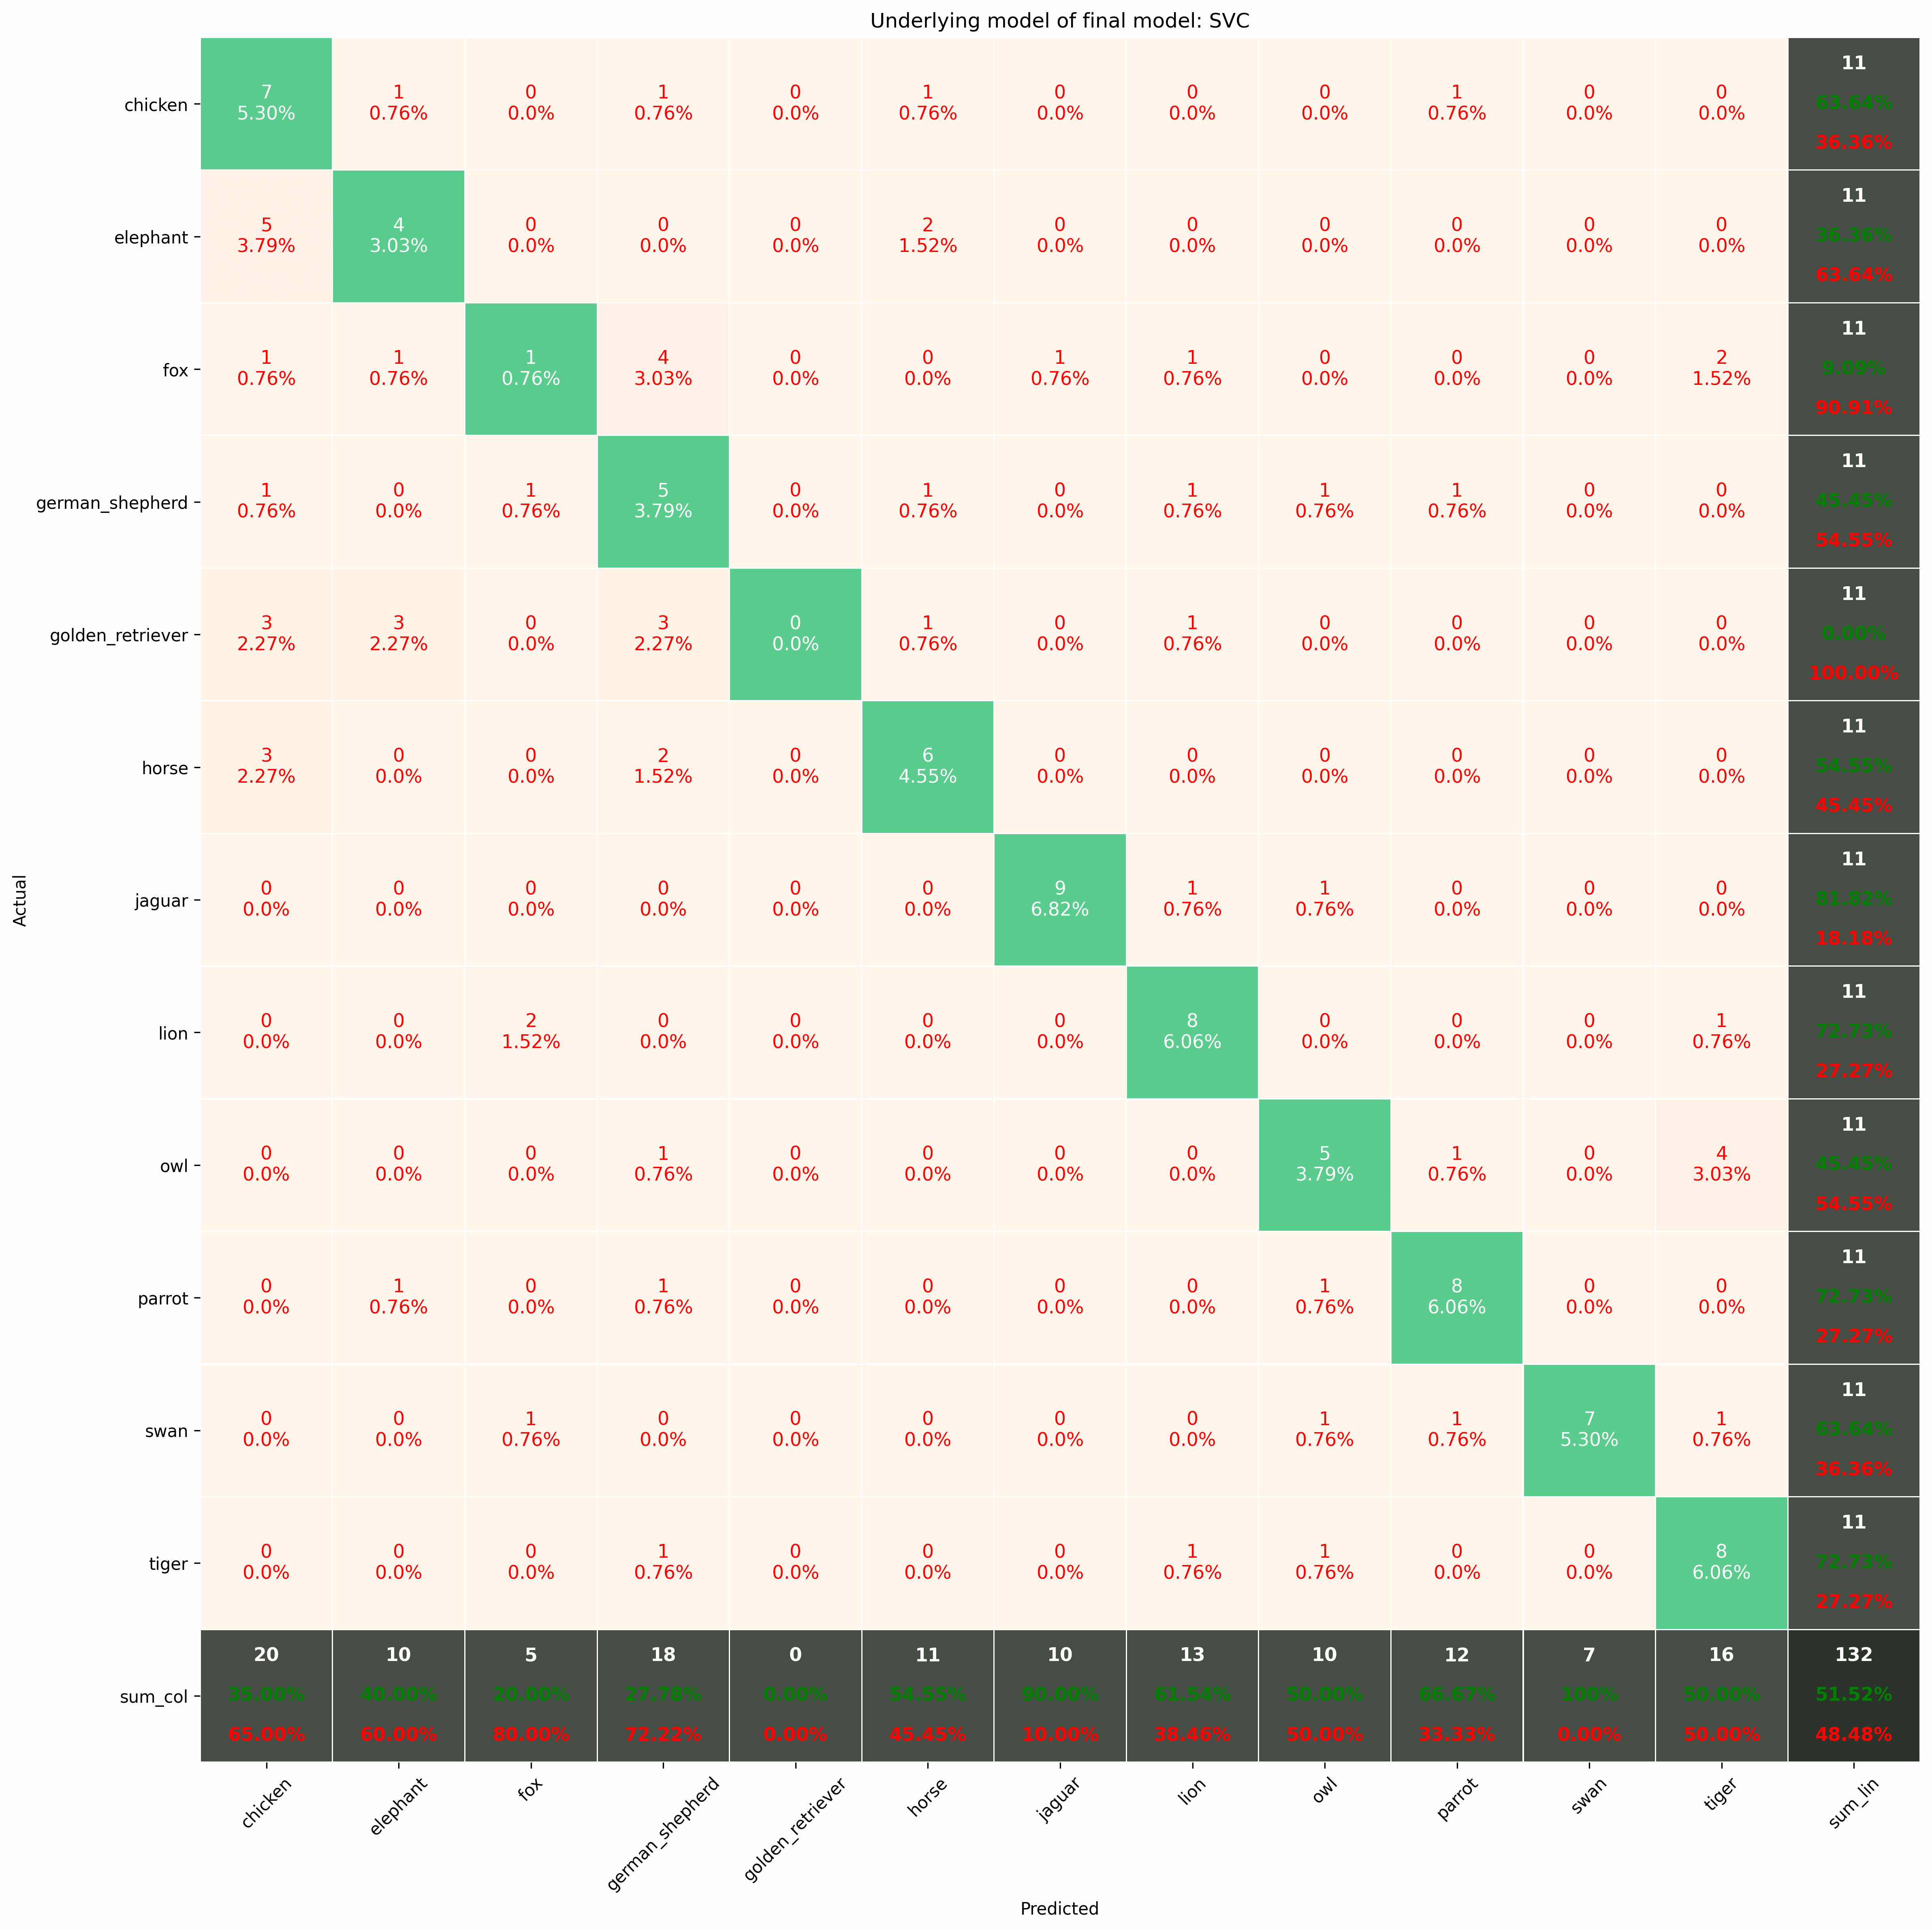
\includegraphics[width=\textwidth]{images/final/underlying_SVC.png}}
        \captionsetup{width=0.9\linewidth}
        \captionsetup{justification=centering}
        \caption{CM of the final model's underlying SVC model.}
    \end{subfigure}
    \hspace{1cm}
    \begin{subfigure}{.45\textwidth}
        \centering
        \fbox{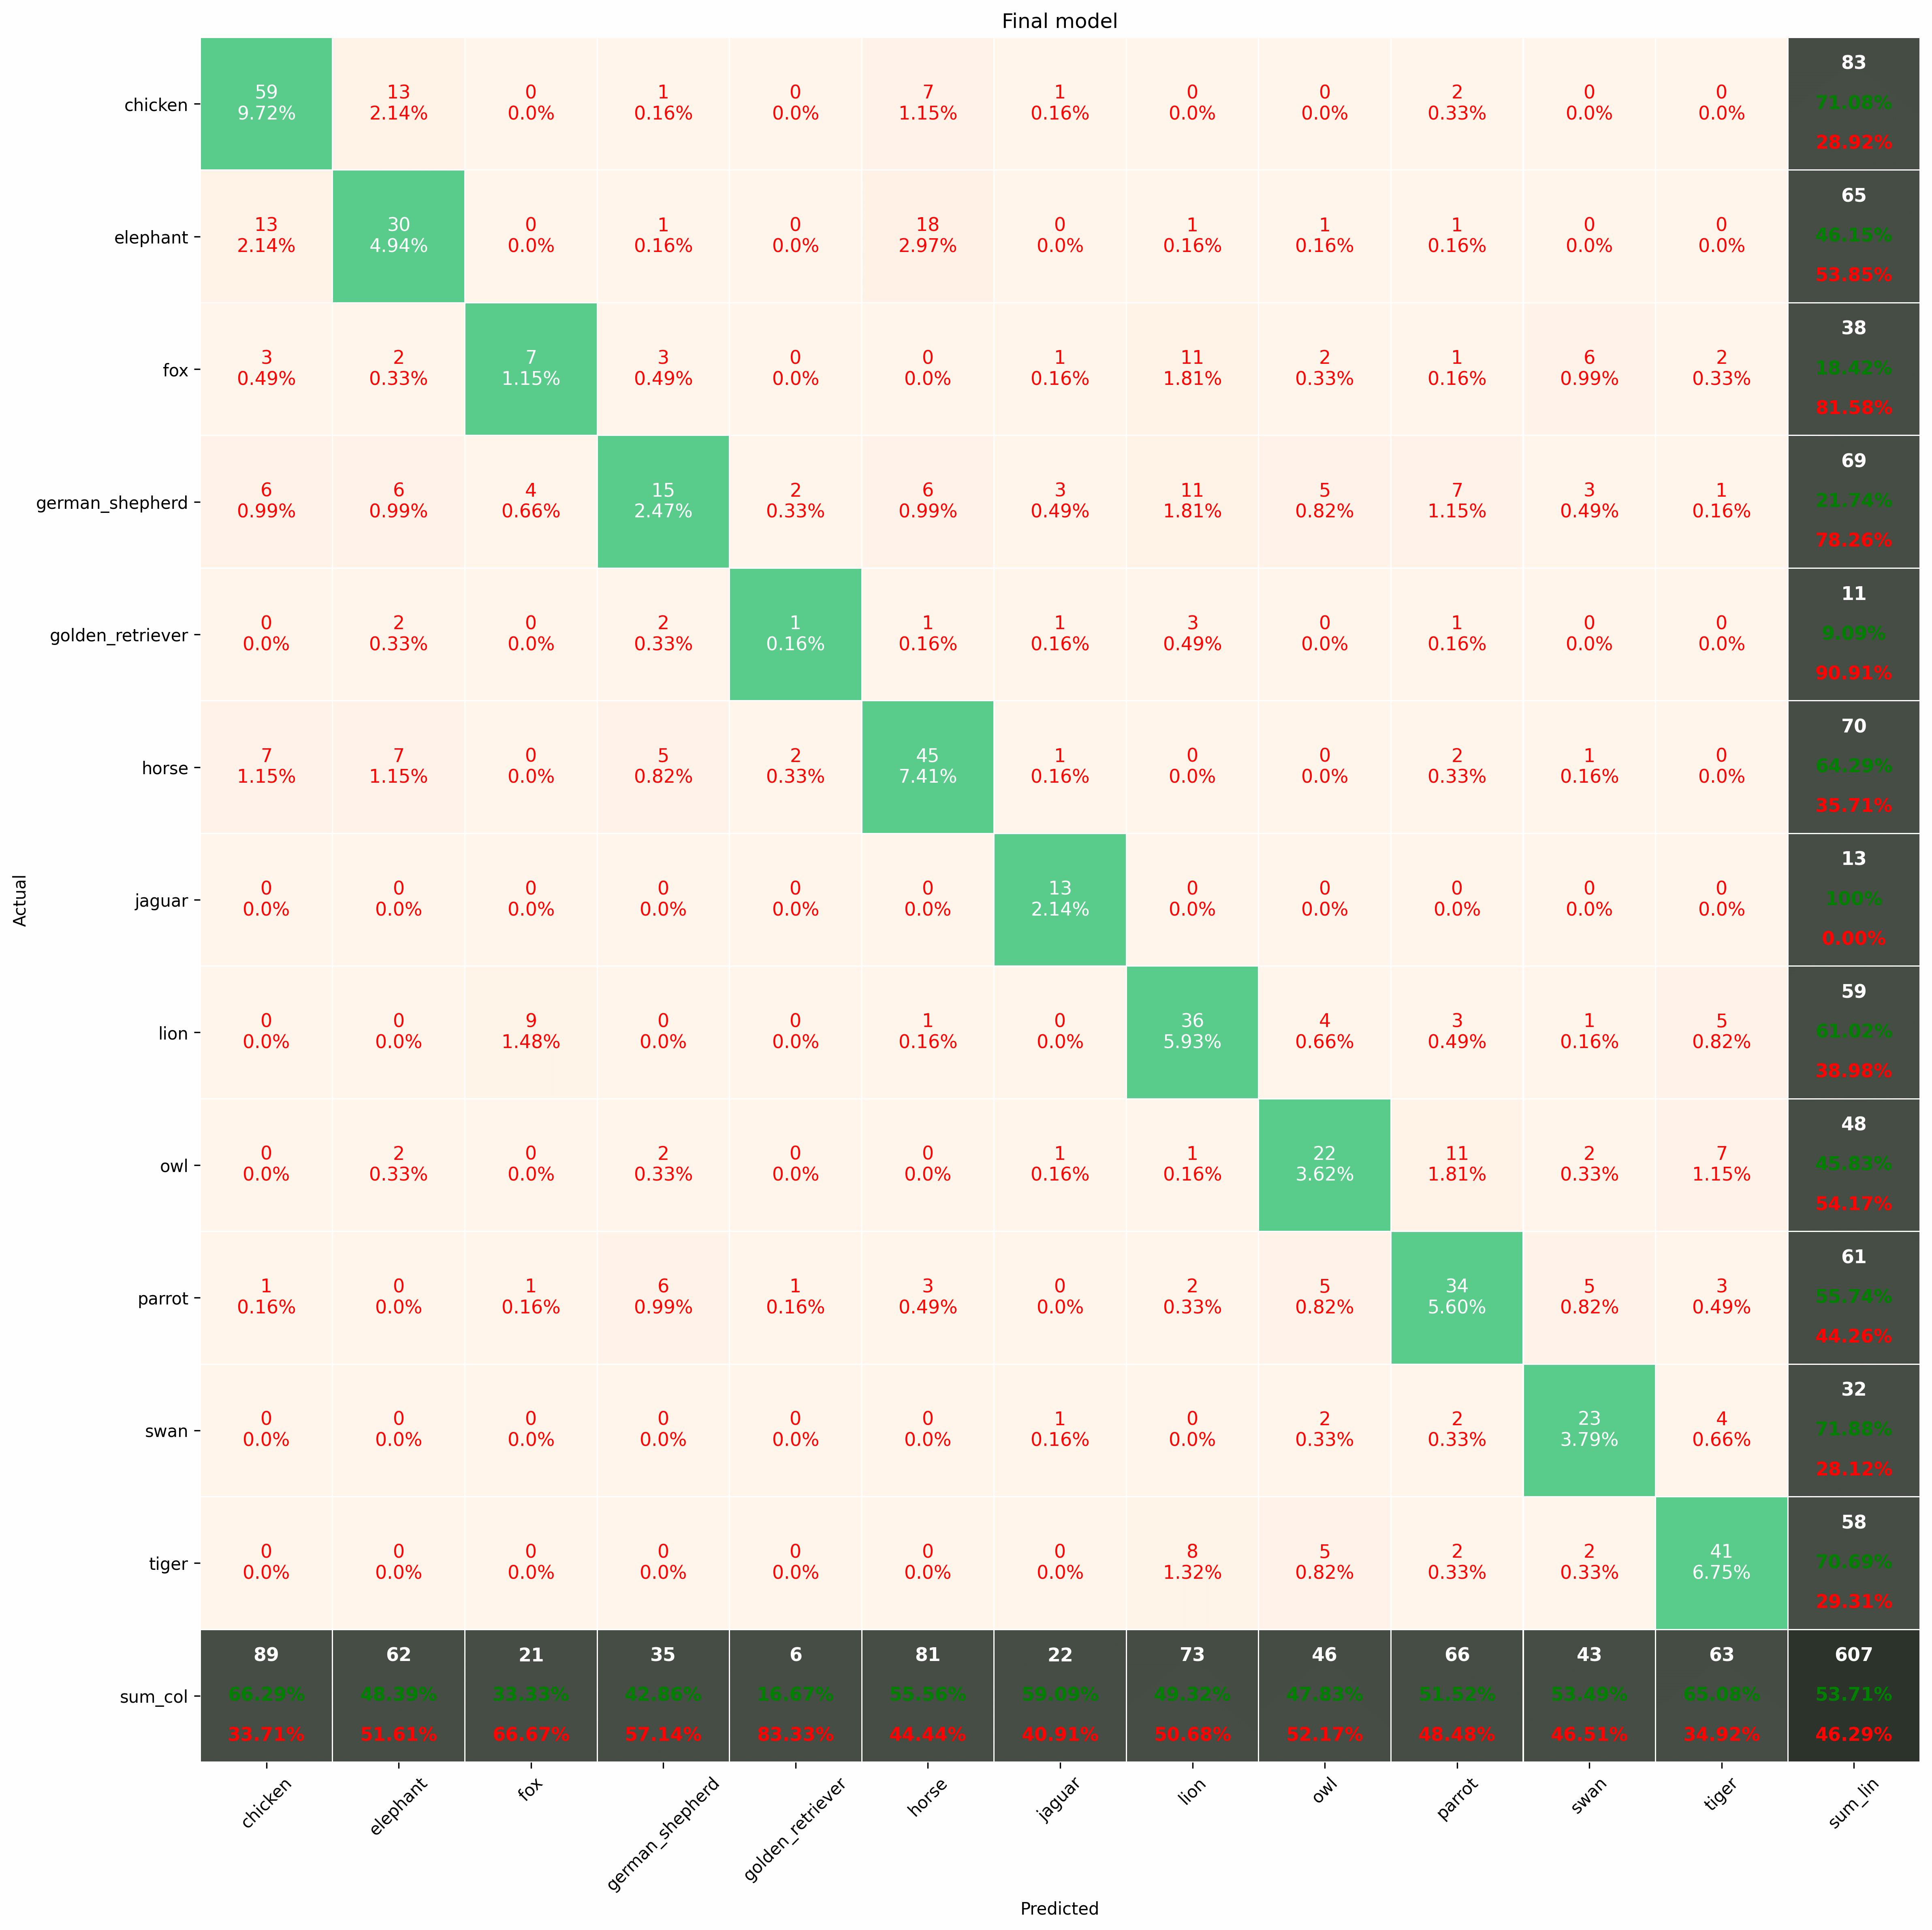
\includegraphics[width=\textwidth]{images/final/final_cm.png}}
        \captionsetup{width=0.9\linewidth}
        \captionsetup{justification=centering}
        \caption{CM of the final model.}
    \end{subfigure}
    \captionsetup{width=0.8\linewidth}
    \captionsetup{justification=centering}
    \caption{Confusion matrices of the final model and its underlying SVC model.}
    \label{fig:final_model_cm}
\end{figure*}